% !TEX encoding = UTF-8
% !TEX TS-program = pdflatex
% !TEX root = ../tesi.tex

%**************************************************************
\chapter{Svolgimento}
\label{cap:svolgimento}
%**************************************************************

\intro{Il presente capitolo descrive le varie fasi dello sviluppo dell'applicativo.}

\section{Pianificazione}
	\subsection{Modello di sviluppo}
	Come modello per la gestione del progetto ho adottato la metodologia \gls{agileg} Scrum. 	
 Tale modello mi ha permesso di poter rispondere con velocità e flessibilità alle esigenze e ai feedback  degli stakeholder, in questo caso il tutor aziendale e il Dipartimento di Amministrazione. \\
	
	\begin{figure}[H]
		\centering
		
\includegraphics[width=0.8\linewidth]{immagini/agile}
		\caption{Metologia Agile}
		\label{fig:agile}
	\end{figure}
	
	Il modello \emph{Agile} prevede iterazioni continue, della durata massima di due settimane,
	entro le quali si susseguono attività di:
	\begin{enumerate}
		\item analisi dei requisiti che emergono dall’interazione con gli stakeholder;
		\item pianificazione delle funzionalità da includere nello sprint e loro suddivisione in task;
		\item progettazione delle funzionalità da implementare nell’iterazione corrente;
		\item codifica e sviluppo delle funzionalità previste;
		\item verifica;
		\item rilascio;
		\item monitoraggio continuo e verifica dello stato dell’applicazione.
	\end{enumerate}
	
	Il punto di partenza di ogni iterazione è il risultato raggiunto con il precedente e il feedback
	ricevuto tramite la presentazione della soluzione raggiunta fin’ora agli stakeholder.
	
	Al seguente indirizzo è possibile visionare i principi del modello di ciclo di sviluppo
	Agile:
		\begin{center}
		\url{http://agilemanifesto.org/iso/it/principles.html}
		\end{center}
	
	\subsection{Pianificazione settimanale}
	La duranta dello stage è stata di 8 settimane quindi ho pianificato 4 sprint della durata di due settimane ognuno in cui ho eseguito le seguenti operazioni:
	\begin{enumerate}
		\item studio delle tecnologie, degli strumenti di sviluppo e del sotware gestionale esistente;
		\item progettazione, codifica e testing del modulo Banche;
		\item progettazione, codifica e testing del modulo Fatture Attive;
		\item progettazione, codifica e testing del modulo Fatture Passive.
	\end{enumerate}

%\section{Analisi dei requisiti}
%**************************************************************
Nella fase di analisi dei requisiti, ho avuto modo di discutere a fondo con il tutor
aziendale le funzionalità che il prodotto doveva rendere disponibili, aiutandoci anche con lo studio delle funzionalità disponibili nel vecchio gestionale ancora operativo.

Nella tabelle che seguono verranno presentati i principali requisiti individuati
durante l’analisi del problema e della soluzione già implementata nel vecchio applicativo, discussi con il tutor e il Dipartimento di Amministrazione.
Ogni requisito individuato avrà un codice identificativo univoco così formato:
Il codice dei requisiti è così strutturato R(F/Q/V)(N/D/O) dove:
\begin{enumerate}
	\item[R =] requisito;
    \item[F =] funzionale;
    \item[Q =] qualitativo;
    \item[V =] di vincolo;
    \item[N =] obbligatorio (necessario);
    \item[D =] desiderabile;
    \item[Z =] opzionale.
\end{enumerate}

\newpage

\begin{table}%
\caption{Tabella del tracciamento dei requisti funzionali}
\label{tab:requisiti-funzionali}
\begin{tabularx}{\textwidth}{lXl}
\hline\hline
\textbf{Requisito} & \textbf{Descrizione} & \textbf{Importanza}\\
\hline
RFN-1     & L'interfaccia permette di configurare il tipo di sonde del test & Obbligatorio \\
\hline
\end{tabularx}
\end{table}%

\begin{table}%
\caption{Tabella del tracciamento dei requisiti qualitativi}
\label{tab:requisiti-qualitativi}
\begin{tabularx}{\textwidth}{lXl}
\hline\hline
\textbf{Requisito} & \textbf{Descrizione} & \textbf{Importanza}\\
\hline
RQD-1    & Le prestazioni del simulatore hardware deve garantire la giusta esecuzione dei test e non la generazione di falsi negativi & Obbligatorio \\
\hline
\end{tabularx}
\end{table}%

\begin{table}%
\caption{Tabella del tracciamento dei requisiti di vincolo}
\label{tab:requisiti-vincolo}
\begin{tabularx}{\textwidth}{lXl}
\hline\hline
\textbf{Requisito} & \textbf{Descrizione} & \textbf{Importanza}\\
\hline
RVO-1    & La libreria per l'esecuzione dei test automatici deve essere riutilizzabile & - \\
\hline
\end{tabularx}
\end{table}%


\section{Strumenti e Tecnologie Utilizzate}
	Per lo sviluppo del progetto ho utilizzato le seguenti tecnologie:
		\begin{itemize}
			\item \hyperref[tec:django]{Django e Django REST Framework};
			\item \hyperref[tec:angular]{Angular};
			\item \hyperref[tec:web]{HTML 5, CSS3 e Bootstrap};
			\item \hyperref[tec:git]{Git};
			\item  gli \hyperref[tec:intellij]{IDE Jetbrains}.
		\end{itemize}
	
	\subsection{Django e Django REST Framework}
	\label{tec:django}
	Django è un framework di alto livello, gratuito e open source per lo sviluppo in modo veloce e pulito di applicazioni web in Python.\\ \\
	Il framework è composto da:
	\begin{itemize}
	\item un \gls{orm} che consente di mappare lo schema di un database relazionele su cui vengono eseguite le operazioni in modelli definiti in Django; inoltre consente la generazione dei modelli (classi in linguaggio Python che rappresentano le tabelle) a partire dallo schema del database e viceversa;
	\item un dispatcher URL basato sulle espressioni regolari in grado di effettuare il parsing degli indirizzi che vengono inseriti secondo delle specifiche anche complesse, cioè comprendendo parametri o espressioni regolari;
	\item un sistema di view per l’elaborazione delle richieste del client;
	\item un sistema di template per la visualizzazione dei contenuti.
	\end{itemize}
	
	Django REST Framework è un insieme di librerie che semplifica la creazione di \gls{apig} offrendo in particolare strumenti per la conversione di dati complessi, ad esempio i risutati delle interrogazioni al database, in tipi di dato nativi di Python che possono essere manipolati e facilmente renderizzati nel formato desiderato.\\
	\begin{figure}[H]
		\centering
		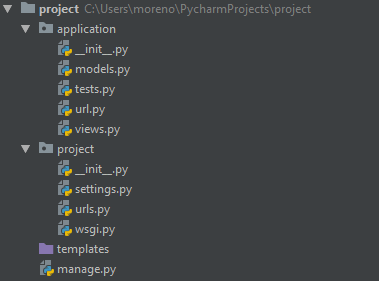
\includegraphics[width=0.6\linewidth]{immagini/django-arch}
		\caption{I file di un'applicazione Django}
		\label{fig:django-arch}
	\end{figure}
	
	Come si può vedere in figura \ref{fig:django-arch} il framework favorisce la sviluppo di applicazioni strutturate in quanto è raccomandato che ogni applicazione sia divisa nei seguenti moduli:
	\begin{itemize}
	\item \textbf{models:} il modulo che contiene le strutture dati che rappresentano le tabelle del database e metodi che rappresentano comportamenti essenziali dei dati che rappresentano.
	\item \textbf{serializers:} il modulo in cui si definiscono le classi che si occupano della conversione dei risultati delle interrogazioni al database in dizionari o liste pronte per la trasmissione e, viceversa, di creare le istanze da inserire nel database a partire da dizionari.
	\item \textbf{views:} il modulo che contiene le definizioni dei servizi del web-service, cioè funzioni che accettano come parametro una richiesta \gls{http} ed eventuali argomenti e ritornano una risposta \gls{http}.
	\item \textbf{urls:} il modulo in cui si definiscono le associazioni tra stringhe oppure espressioni regolari e i metodi contenuti in \textit{views}.
	\item \textbf{tests:} il modulo che contiene la definizione dei test e ne consente l'esecuzione in modo automatico.
	\end{itemize}
	
	\subsection{Angular}
	\label{tec:angular}
	Angular è una piattaforma e un framework open-source per lo sviluppo di applicazioni client in HTML e TypeScript.
	Il framework si basa sui seguenti principi:
	\begin{itemize}
	\item \textbf{Mobile first}: Uno degli obiettivi del nuovo Angular è di proporsi per lo sviluppo di applicazioni Web sia per l’ambiente desktop che per il mobile. Infatti, Angular 2 supporta di default eventi touch e gesture;
	\item \textbf{Modularità}: l’architettura di Angular  è altamente modulare e favorisce la
	scrittura di applicazioni modulari;
	\item \textbf{Prestazioni}: un’attenzione particolare è stata posta sulle prestazioni del framework, dalla riduzione dei tempi di caricamento e boostrapping dell’applicazione, al rilevamento efficiente delle modifiche nel modello dei dati ed alla velocità dei tempi di rendering.
	\end{itemize}

	Un’applicazione Angular è composta dai seguenti tipi di elementi:
	\begin{itemize}
	\item \textbf{Template}: file che contiene la sruttura di base della pagina HTML da mostrare;
	\item \textbf{Component}: classe gestore del template associato e di cui permette il cambiamento dinamicamente;
	\item \textbf{Services}: classi che forniscono funzionalità condivise da più componenti, ad esempio i metodi di interazione con il back-end, per favorire la riusabilità del codice ed evitare duplicazione;
	\item \textbf{Module}: classi che permettono il raggruppamento di componenti correlati logicamente fra loro; a differenza dei servizi ogni componente può far parte di uno e un solo modulo.
	\end{itemize}

	\begin{figure}[H]
		\centering
		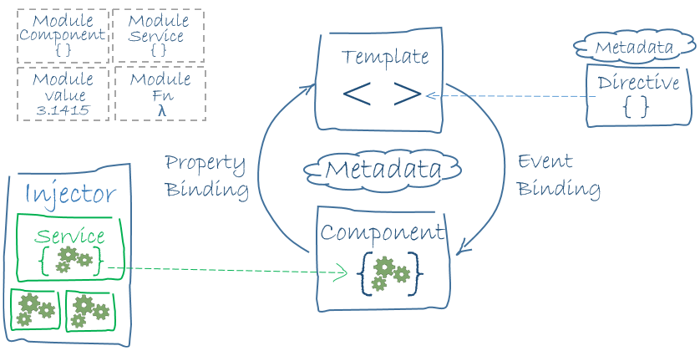
\includegraphics[width=0.8\linewidth]{immagini/angular-arch}
		\caption{Architettura di Angular}
		\label{fig:angular-arch}
	\end{figure}
	
	\subsection{HTML 5, CSS3 e Bootstrap}
	\label{tec:web}
	Per la realizzazione delle pagine web viene utilizzato il linguaggio di markup \gls{html}5
il quale è l’attuale standard di riferimento. Per facilitare la realizzazione del layout
grafico delle pagine e la gestione di alcuni eventi ed animazioni viene utilizzato 
\gls{css}3, abbinato alla vasta libreria offerta da \gls{bootstrapg}\cite{site:bootstrap}.
	
	\subsection{Git}
	\label{tec:git}
	I progetto è soggetto a versionamento attraverso il software Git, un sistema di controllo di versione distribuito, creato da Linus Torvalds nel 2005. \\
Git supporta lo sviluppo non lineare con diramazioni e fusioni rapide e continue
e comprende strumenti specifici per visualizzare e navigare una cronologia di sviluppo.\\
Permette ad ogni sviluppatore una copia locale dell’intera cronologia di sviluppo e le
modifiche vengono importate da un repository ad un altro. \\
Il relativo repository è ospitato su Bitbucket, un servizio di hosting web-based
per progetti che usano i sistemi di controllo versione Mercurial o Git.
	
	\subsection{IntelliJ e derivati}
	\label{tec:intellij}
	Per l'attività di codifica dell'applicativo ho scelto di utilizzare PyCharm e WebStorm, due prodotti sviluppati da JetBrains come derivazioni di IntelliJ ottimizzate rispettivamento per progetti in Linguaggio Python e progetti Web.\\ \\
	Ho scelto di utilizzare questi IDE perchè offrono i seguenti vantaggi:
	\begin{itemize}
	\item permettono la configurazione del sistema di building in modo semplice;
	\item integrazione con il sistema di versionamento Git; 
	\item contengono un sistema di versionamento integrato che tiene traccia di ogni modifica ad ogni singolo file e da cui è possibile ripristinare lo stato precedente;
		\begin{figure}[H]
			\centering
			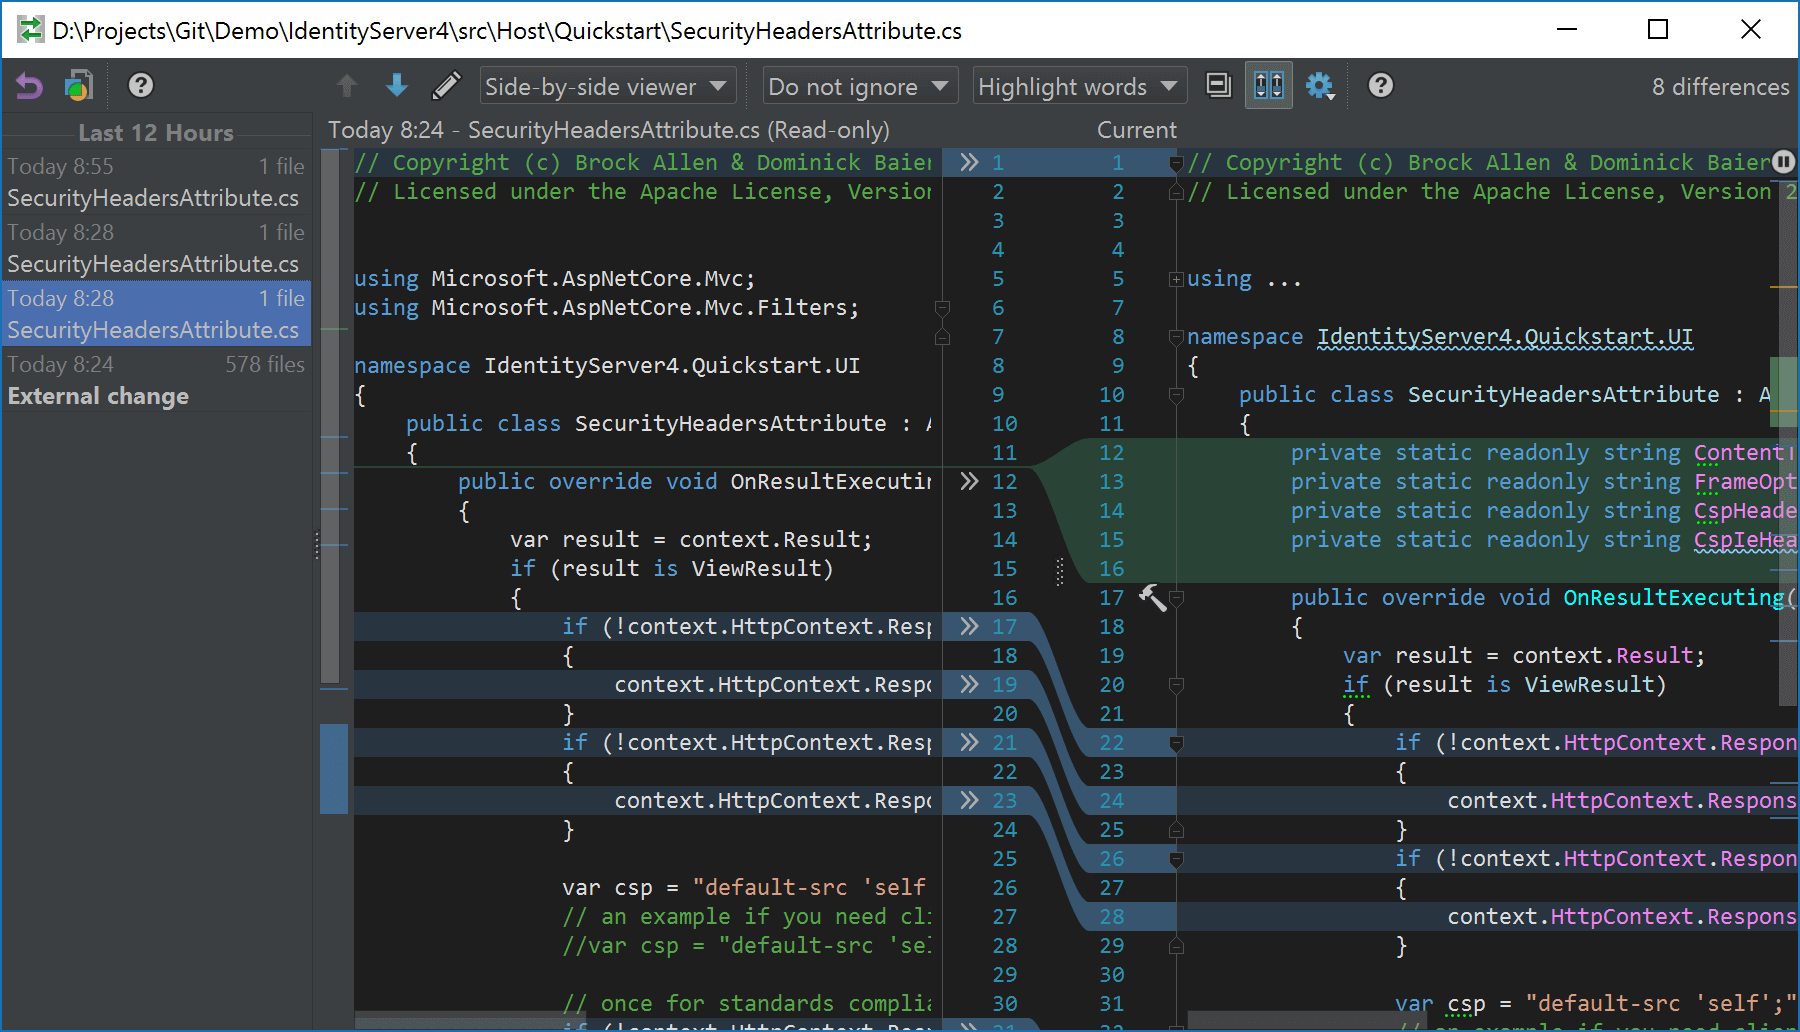
\includegraphics[width=0.8\linewidth]{immagini/ide-history}
			\caption{Il sistema di versionamento integrato dei prodotti JetBrains}
			\label{fig:ide-history}
		\end{figure}
	\item contengono un client ad ingerfaccia grafica per database;
		\begin{figure}[H]
			\centering
			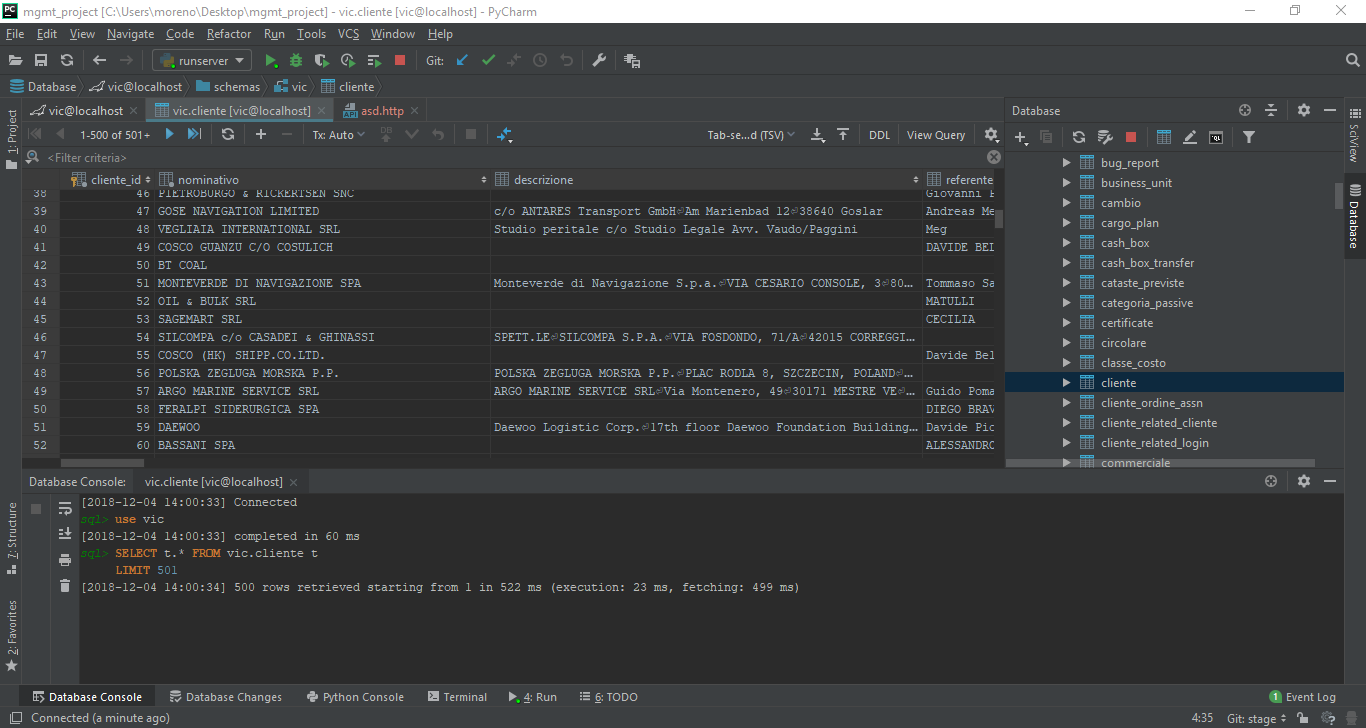
\includegraphics[width=0.8\linewidth]{immagini/ide-database}
			\caption{Il sistema di navigazione di database}
			\label{fig:ide-history}
		\end{figure}
	\item contengono un client per \gls{apig} \gls{restg} con possibilità di effetturare test inserendo asserzioni sul risultato;
		\begin{figure}[H]
			\centering
			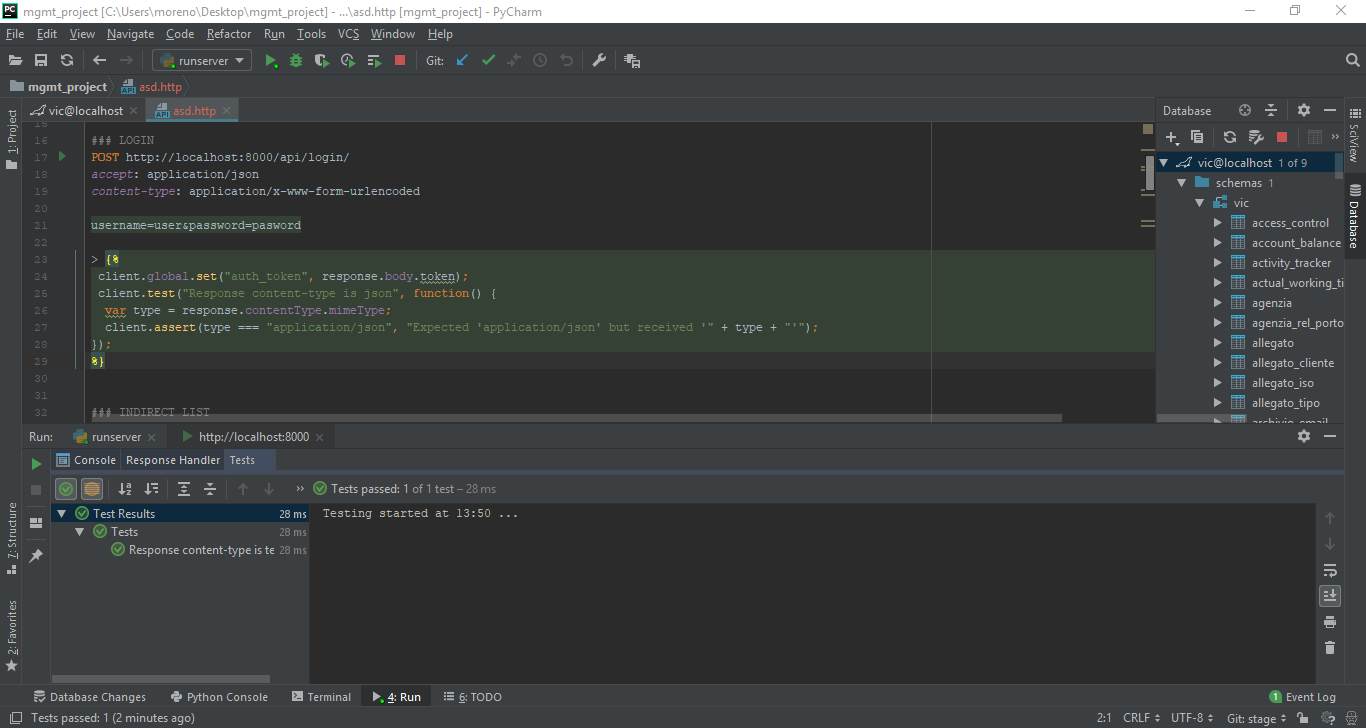
\includegraphics[width=0.8\linewidth]{immagini/ide-rest}
			\caption{Il client per API REST}
			\label{fig:ide-history}
		\end{figure}
	\item integra uno strumento di analisi statica del codice con segnalazione degli errori.
		\begin{figure}[H]
			\centering
			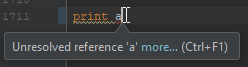
\includegraphics[width=0.5\linewidth]{immagini/ide-error}
			\caption{Esempio di errore segnalato dall'IDE}
			\label{fig:ide-error}
		\end{figure}
	\end{itemize}

\section{Progettazione}
	\subsection{Progettazione Architetturale}
Ho seguito il principio di progettazione \emph{Separation of Concerns} (traduzione: separazione delle responsabilità) al fine di dividere l'applicativo in più parti logicamente separate e quindi più semplici. \\ \\
Il sitema risultante, ad alto livello, è diviso in due componenti principali:
	\begin{itemize}
		\item \textbf{Front-end}: si occupa di gestire l'interazione con l'utente ed è responsabile dell'acquisizione dei dati di ingresso e della loro elaborazione in modo tale da renderli utilizzabili dal back end;
		\item \textbf{Back-end}: si occupa interagire con il database, elaborare i dati e mettere a disposizione i servizi al client ( il front-end).
	\end{itemize}
	
	Le due componenti sono indipendenti tra loro e comunicano tramite \gls{apig} \gls{restg} nelle quali vengono scambiati dati in formato \gls{json}.

	\begin{figure}[H]
		\centering
		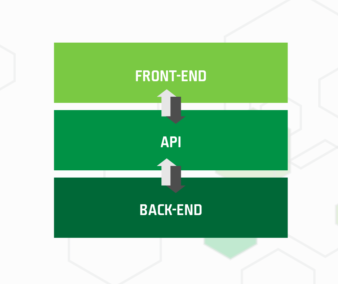
\includegraphics[width=0.8\linewidth]{immagini/arch}
		\caption{Architettura di alto livello}
		\label{fig:arch}
	\end{figure}

	\subsection{Back-end}
	Il back-end dell'applicativo è stato realizzato utilizzando i framework \hyperref[tec:django]{Django e Django REST Framework}\cite{site:djangorest}.\\
	Esso è suddiviso in tre moduli che rispecchiano le tre sezioni dellapplicativo da realizzare:
	\begin{itemize}
		\item \textbf{banche};
		\item \textbf{fatture\_attive};
		\item \textbf{fatture\_passive}.
	\end{itemize}
	
	Ognuno di questi moduli contiene al suo interno tutti i sottomoduli descritti approfonditamente nella sezione \hyperref{tec:django} in modo da tenere separati oggetti non correlati e quindi facilitarne la manutenibilità e il riuso:
	\begin{itemize}
		\item models;
		\item serializers;
		\item views;
		\item urls;
		\item tests.
	\end{itemize}

	\subsection{Front-end}
	L’utilizzo del framework Angular mi hanno da subito imposto una visione predefinita dell’architettura dell’applicazione. \\
	Seguendo le direttive dettate dall'utilizzo del framework Angular, spiegate alla sezione \hyperref{tec:angular}, ho diviso l'applicativo in due \emph{package}:
	\begin{itemize}
		\item \textbf{services} che si occupa di contenere tutti i servizi, cioè le classi che forniscono funzionalità condivise da più componenti, nello specifico i metodi di interazione con il back-end;
		\item \textbf{views} che contiene tutti i moduli, i componenti e i template ad essi associati per la per la realizzazione delle pagine.
	\end{itemize}
	
	\subsubsection{Services}
	Questa parte contiene le classe che rappresentano i servizi che permettono di accedere alle \gls{apig} offerte dal corrispondente modulo del back-end:
	\begin{itemize}
		\item \textbf{BancheService}, che permette di accedere alle \gls{apig} offerte dal corrispondente modulo \textit{banche};
		\item \textbf{FattureAttiveService}, che permette di accedere alle \gls{apig} offerte dal corrispondente modulo \textit{fatture\_attive};
		\item \textbf{FatturePassiveService}, che permette di accedere alle \gls{apig} offerte dal corrispondente modulo \textit{fatture\_passive};
	\end{itemize}
	
	\subsubsection{Views}
	Questa parte contiene la gerarchia dei moduli e dei componenti in essi contenuti.\\
	Nello specifico, procedendo in ordine top-down, sono contenuti i seguenti moduli:
	\begin{itemize}
		\item \textbf{BancheModule}, che dipende dal servizio \emph{BancheService} e contiene tutti i componenti necessari ad offrire all'utente le funzionalità facenti parte del \hyperref[mod:banche]{Modulo Banche};
		\item \textbf{FattureAttiveModule}, che dipende dal servizio \emph{FattureAttiveService} e contiene tutti i componenti necessari ad offrire all'utente le funzionalità facenti parte del \hyperref[mod:fa]{Modulo Fatture Attive};
		\item \textbf{FatturePassiveModule}, che dipende dal servizio \emph{FatturePassiveService} e contiene tutti i componenti necessari ad offrire all'utente le funzionalità facenti parte del \hyperref[mod:fp]{Modulo Fatture Passive}.
	\end{itemize}
	
	Al fine di evitare inutili dipendenze e mantenere una struttura del progetto semplice e coerente, è stato scelto che i template associati ai componenti:
	\begin{itemize}
		\item risiedano nella stessa cartella del loro componente associato;
		\item abbiano lo stesso nome del componente associato.
	\end{itemize}
	
	\begin{figure}[H]
		\centering
		
\includegraphics[width=0.4\linewidth]{immagini/angular-comp}
		\caption{Esempio di cartella contenente un componente}
		\label{fig:angular-arch}
	\end{figure}
	
	\subsection{Comunicazione tra front-end e back-end}
La comunicazione tra il back-end e il front-end avviene tramite un insieme di \gls{apig} che
il primo mette a disposizione del secondo seguendo i principi \gls{restg}.
Lo stile architetturale \gls{restg} prescrive che lo stato in un’applicazione le sue funzionalità
siano interpretati come risorse web univoche e accessibili tramite un \gls{url} attraverso il protocollo \gls{http} o il protocollo \gls{soap}.
\\ \\

L’approccio architetturale  \gls{restg} è definito dai seguenti vincoli applicati ad un’architettura:
\begin{itemize}
\item \textbf{Client-server}: un insieme di interfacce uniformi separa il client dal server in
modo da ridurre l’accoppiamento tra le componenti del sistema;
 \item \textbf{Stateless}: la comunicazione client–server è vincolata in modo
che nessun contesto client venga memorizzato sul server tra le richieste. Ogni
richiesta da ogni client contiene tutte le informazioni necessarie per richiedere il
servizio, e lo stato della sessione è contenuto sul client;
\item \textbf{Cacheable}: i client possono fare caching delle risposte;
\item \textbf{Layered system}: i client non sono tenuti a conoscere quale livello del sistema
server stanno interrogando.
\end{itemize}
Tale architettura è molto semplice, facile da implementare e riduce notevolmente l’accoppiamento tra client e server;
per questi motivi è diffusa nelle applicazioni web.

\section{Verifica e Validazione}

	\subsection{Verifica}
	Durante l’intera attività di sviluppo ho verificato che quanto svolto fosse conforme alle
	attese del mio tutor e dei membri del Dipartimento di Amministrazione. Per far ciò ho attuato molte prove pratiche sulle
	funzionalità implementate, per assicurarmi che funzionassero in modo adeguato. \\ \\
	L’azienda ha preferito utilizzare le prove manuali piuttosto di dedicare tempo alla progettazione e codifica di un sitema automatizzato di verifica,
	in modo che potessi concentrarmi sull’adeguare il prodotto secondo le loro esigenze. \\ 
	Grazie al lavoro svolto in fase di configurazione dell’ambiente di lavoro, ho potuto
	testare velocemente l’applicazione in locale con la base di dati contenente i dati reali.
	
	\subsubsection{Analisi Statica}
	Per l’attività di verifica durante tutto l’arco di sviluppo del progetto ho utilizzato strumenti di analisi
	integrati negli IDE in modo da controllare che il codice fosse uniforme, scritto secondo dei
	buoni canoni e che rispettasse opportuni standard di codifica in base al linguaggio, altrimenti segnalati con \emph{warning}.
	
	\begin{figure}[H]
		\centering
		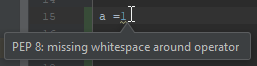
\includegraphics[width=0.5\linewidth]{immagini/pyc-warning}
		\caption{Esempio di warning dovuto al non rispetto delle norme di sintassi}
		\label{fig:pycarm-warning}
	\end{figure}
	
	In particolare tutto il codice scritto in linguaggio Python rispetta le convenzioni \textit{PEP8}, reperibili al link:
	\begin{center}
		\url{https://www.python.org/dev/peps/pep-0008/}
	\end{center}

	Invece il codice in linguaggio TypeScript è stato analizzando utilizzando il tool opensource TSLint, reperibile al link:
	\begin{center}
		\url{https://palantir.github.io/tslint/}
	\end{center}
	
	\subsection{Validazione}
Il processo di validazione ha lo scopo di accertare che il prodotto finale corrisponda alle attese soddisfando tutti i requisiti prefissati inizialmente e va a dimostrare che il prodotto dello stage si comporti come specificato. Occorre provare che fornisce tutte le funzionalità, le prestazioni, l’affidabilità richieste e che non fallisca. \\

\subsubsection{Test di accettazione}
Segue un elenco dei test di accettazione effettuati durante il mio stage.

\begin{table}[H]
\caption{Tabella dei test di Accettazione}
\begin{tabularx}{\textwidth}{lXl}
\hline\hline
\textbf{Test} & \textbf{Descrizione} & \textbf{Esito}\\
\hline
TA-1 & Visualizzazione della lista delle banche associata alla sede & Superato\\
TA-2 & Visione di tutti i movimenti di un conto corrente & Superato\\
TA-3 & Aggiornamento del saldo di un conto corrente & Superato\\
TA-4 & Caricamento di un estratto conto & Superato\\
TA-5 & Visione di di un estratto conto & Superato\\
TA-6 & Inserimento di un movimento bancario & Superato\\
TA-7 & Modifica di movimento bancario & Superato\\
TA-8 & Rimozione di movimento bancario & Superato\\
TA-9 & Generazione del file \emph{Pdf} della lista dei movimenti bancari & Superato\\
TA-10 & Generazione del file \emph{xls} della lista dei movimenti bancari & Superato\\
TA-11 & Visualizzazione della lista degli ordini completati e non ancora fatturati & Superato\\
TA-12 & Creazione di una fattura a partire dagli ordini completati & Superato\\
TA-13 & Ricerca di fatture attraverso il numero di ordine & Superato\\
TA-14 & Ricerca di fatture attraverso il nome della nave & Superato\\
TA-15 & Creazione di una fattura attiva & Superato\\
TA-16 & Modifica di una fattura attiva & Superato\\
TA-17 & Rimozione di una fattura attiva & Superato\\
TA-18 & Visualizzazione della lista di fatture non ancora inviate al cliente; & Superato\\
TA-19 & Generazione di file in formato \emph{Pdf} corrispondenti alle fatture; & Superato\\
TA-20 & Invio di fatture al cliente tramite email & Superato\\
TA-21 & Visualizzazione dello scadenziario delle fatture emesse da incassare & Superato\\
TA-22 & Visualizzazione della lista delle fatture passive dirette non pagate raggruppate per fornitore & Superato\\
TA-23 & Visualizzazione della lista delle passive indirette & Superato\\
TA-24 & Visualizzazione del dettaglio singola fattura passiva & Superato\\
TA-25 & Modifica di una singola fattura passiva & Superato\\
TA-26 & Eliminazione di una fattura passiva & Superato\\
TA-27 & Pagamento e generazione del movimento bancario associato a una fattura passiva & Superato\\
\hline
\end{tabularx}
\end{table}%

\subsubsection{Validazione esterna}
Al termine dello stage in presenza del tutor è stata effettuata una presentazione del lavoro svolto durante il periodo di stage e sono stati eseguiti tutti i test sopra elencati.\\
\paragraph{}
Tutti i test in sede di validazione esterna sono stati superati con
successo e la presentazione è terminata con demo che dimostrava l’effettiva copertura di tutti i requisiti pianificati ed il soddisfacimento di tutte le funzionalità richieste.\\
